\documentclass[twoside,twocolumn]{article}

\usepackage{blindtext} % Package to generate dummy text throughout this template 
\usepackage{graphicx}
\usepackage[sc]{mathpazo} % Use the Palatino font
\usepackage[T1]{fontenc} % Use 8-bit encoding that has 256 glyphs
\linespread{1.05} % Line spacing - Palatino needs more space between lines
\usepackage{microtype} % Slightly tweak font spacing for aesthetics

\usepackage[english]{babel} % Language hyphenation and typographical rules

\usepackage[hmarginratio=1:1,top=32mm,columnsep=20pt]{geometry} % Document margins
\usepackage[hang, small,labelfont=bf,up,textfont=it,up]{caption} % Custom captions under/above floats in tables or figures
\usepackage{booktabs} % Horizontal rules in tables
\usepackage{graphicx}
\usepackage{lettrine} % The lettrine is the first enlarged letter at the beginning of the text

\usepackage{enumitem} % Customized lists
\setlist[itemize]{noitemsep} % Make itemize lists more compact

\usepackage{abstract} % Allows abstract customization
\renewcommand{\abstractnamefont}{\normalfont\bfseries} % Set the "Abstract" text to bold
\renewcommand{\abstracttextfont}{\normalfont\small\itshape} % Set the abstract itself to small italic text

\usepackage{titlesec} % Allows customization of titles

\titleformat{\section}[block]{\large\scshape\centering}{\thesection.}{1em}{} % Change the look of the section titles
\titleformat{\subsection}[block]{\large}{\thesubsection.}{1em}{} % Change the look of the section titles

\usepackage{fancyhdr} % Headers and footers
\pagestyle{fancy} % All pages have headers and footers
\fancyhead{} % Blank out the default header
\fancyfoot{} % Blank out the default footer
\fancyhead[C]{Herramientas de gestión de pruebas $\bullet$ Noviembre 2021 $\bullet$ } % Custom header text
\fancyfoot[RO,LE]{\thepage} % Custom footer text

\usepackage{titling} % Customizing the title section

\usepackage{hyperref} % For hyperlinks in the PDF

%----------------------------------------------------------------------------------------
%	TITLE SECTION
%----------------------------------------------------------------------------------------
\providecommand{\keywords}[1]{
  \small	
  \textbf{\textit{\quad \quad Keywords: }} #1}

\providecommand{\pclave}[1]{
  \small	
  \textbf{\textit{\quad \quad Palabras Clave: }} #1}

%Idiomas: \selectlanguage{english} \selectlanguage{spanish}

\begin{document}

\title{Trabajo Encargado N°1: Herramientas de gestión de pruebas}

\begin{titlepage}
\begin{figure}[htb]
\begin{center}

\includegraphics[width=5cm]{imagenes/logo.png}
\end{center}
\end{figure}
\vspace*{-0.25in}
\begin{center}
\large{UNIVERSIDAD PRIVADA DE TACNA}\\
\vspace*{-0.025in}
INGENIERIA DE SISTEMAS  \\

\vspace*{0.5in}
\begin{large}
TITULO:\\
\end{large}

\vspace*{0.1in}
\begin{Large}
\textbf{Herramientas de gestión de pruebas} \\
\end{Large}

\vspace*{0.3in}
\begin{Large}
\textbf{CURSO:} \\
\end{Large}

\vspace*{0.1in}
\begin{large}
CALIDAD Y PRUEBAS DE SOFTWARE\\
\end{large}

\vspace*{0.3in}
\begin{Large}
\textbf{DOCENTE:} \\
\end{Large}

\vspace*{0.1in}
\begin{large}
 Mag. Ing. Patrick Cuadros Quiroga\\
\end{large}

\vspace*{0.2in}
\vspace*{0.1in}
\begin{large}

Integrantes: \\
\begin{flushleft}
Martinez Yufra, Ericka Esther\hfill(2018000368) \\
Huillca Aroni, Alfredo\hfill(2018060903)\\
Gorbeño Mamani, Diego Manuel\hfill(2018000354)\\
Loza flore, Midwar Henry \hfill(2017059592)\\
Pomez Huanca Andre Miguel\hfill(2017059537)\\
Anco Copaja, Brian Sebastian\hfill(2018000359)\\

\end{flushleft}
\end{large}

\vspace*{0.1in}
\begin{large}
Tacna - Perú\\
2021
\end{large}
\end{center}
\end{titlepage}

\setlength{\droptitle}{-4\baselineskip} % Move the title up

\pretitle{\begin{center}\Huge\bfseries} % Article title formatting
\posttitle{\end{center}} % Article title closing formatting
\title{Herramientas de gestión de pruebas} % Article title

\date{\today} % Leave empty to omit a date                     
\renewcommand{\maketitlehookd}{%

}

%----------------------------------------------------------------------------------------



% Print the title
\maketitle

%----------------------------------------------------------------------------------------
%	ARTICLE CONTENTS
%----------------------------------------------------------------------------------------

\section{Resumen}

\lettrine[nindent=0em,lines=3]{C}on el auge que han tenido las aplicaciones basadas en la web y en la nube, han surgido numerosas herramientas de software que nos permiten gestionar diversas tareas, hoy en día las herramientas digitales juegan un papel fundamental en el desarrollo de proyectos de software. Estas herramientas, permiten evidenciar la vulnerabilidad, calidad, ingeniería social, cifrado, normas legales y entre otros aspectos dependiendo del software que se pretenda realizar.  A menudo tiene varias capacidades, tales como gestionar los productos de soporte de pruebas, planificación de pruebas, registro de resultados, seguimiento del proceso, gestión de incidencias y generación de informes de las pruebas. 

Este artículo presenta una metodología y el conjunto de herramientas utilizado para la automatización de las pruebas funcionales de software. Algunos ejemplos son: Selenium, Eclipse, Azure Devops, AWS Codepipeline, Google Code Build, Github Actions, etc. Lo que actualmente se logra con las pruebas funcionales hechas en la etapa de desarrollo es el logro de un servicio informático      de primera calidad. Este proceso es una parte muy importante y crítica dentro del proceso de desarrollo de software, y debe realizarse con la mayor eficacia y la mejor eficiencia. 




%------------------------------------------------

\section{Abstract}


With the rise of web and cloud-based applications, numerous software tools have emerged that allow us to manage various tasks, today digital tools play a fundamental role in the development of software projects. These tools allow evidence of vulnerability, quality, social engineering, encryption, legal regulations and among other aspects depending on the software that is intended to be made. It often has multiple capabilities, such as managing test support products, test planning, results recording, process tracking, incident management, and test reporting.

This article presents a methodology and the set of tools used for the automation of software functional tests. Some examples are: Selenium, Eclipse, Azure Devops, AWS Codepipeline, Google Code Build, Github Actions, etc. What is currently being achieved with the functional tests carried out in the development stage is the achievement of a first quality computer service. This process is a very important and critical part of the software development process, and it must be done as effectively and efficiently as possible.




%------------------------------------------------
\section{Introduccion}

Las pruebas de software (en inglés software testing) son las investigaciones empíricas y técnicas cuyo objetivo es proporcionar información objetiva e independiente sobre la calidad del producto a la parte interesada o stakeholder.  

Es una actividad más en el proceso de control de calidad. Las pruebas son básicamente un conjunto de actividades dentro del desarrollo de software. Dependiendo del tipo de pruebas, estas actividades podrán ser implementadas en cualquier momento de dicho proceso de desarrollo. Existen distintos modelos de desarrollo de software, así como modelos de pruebas. A cada uno corresponde un nivel distinto de involucramiento en las actividades de desarrollo.  

A continuación, se describirán algunas herramientas para la realización de pruebas de software 


\section{Desarrollo}
\subsection{Conceptos}
\subsubsection{AWS CodeBuild }

\includegraphics[width=7cm, height=5cm]{imagenes/AWS_CodeBuild.png}
AWS CodeBuild es un servicio de integración continua totalmente administrado que compila código fuente, ejecuta pruebas y produce paquetes de software que están listos para implementarse. Con CodeBuild, no necesita aprovisionar, administrar y escalar sus propios servidores de compilación. CodeBuild escala continuamente y procesa múltiples compilaciones al mismo tiempo, por lo que sus compilaciones no se quedan esperando en una cola. 
\subsubsection{GitHub Actions  }
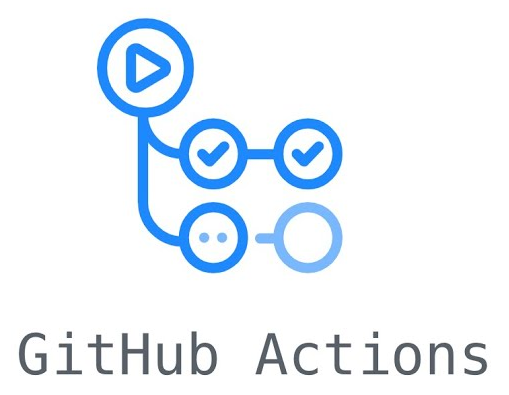
\includegraphics[width=7cm, height=5cm]{imagenes/GithubActions.png}
GitHub es una de las plataformas más utilizadas por los desarrolladores para hosting de repositorios almacenados en la nube. La Integración Continua (IC) es una práctica que requiere de ir añadiendo frecuentemente nuevo código compartido a un repositorio para detectar errores en el menor tiempo posible. Por ello, GitHub propuso, no solo alojar nuestro código en sus repositorios, sino automatizar los pasos de compilación y test de nuestros proyectos. 
\subsubsection{CircleCI }

\includegraphics[width=7cm, height=5cm]{imagenes/CircleCI.png}
CircleCI es la plataforma de integración y entrega continua que ayuda a los equipos de desarrollo a publicar código rápidamente y automatizar la construcción, prueba e implementación. CircleCI se puede configurar para ejecutar canalizaciones muy complejas de manera eficiente con almacenamiento en caché, almacenamiento en caché de la capa de la ventana acoplable, clases de recursos y muchos más. 
\subsection{Comparativa de usabilidad }
\subsubsection{AWS CodeBuild }
Forma sencilla de crear su código con CodePipeline, especialmente con la implementación de pilas de CloudFormation, y la experiencia del usuario no es muy amigable. No requiere ningún permiso especial, ya que está construido dentro del intervalo de su cuenta de AWS normal. Si necesita crear una aplicación móvil en AWS CodeBuild, debe saber que todavía existe un límite con la compilación de macOS. 
Facilita la integración y entrega continuas, ya que AWS CodeBuild pertenece a una familia de servicios de código de AWS que puede utilizar para crear flujos de trabajo de publicación de software completos y automatizados la integración y entregas continuas (CI/CD).  
Con AWS CodeBuild, sus artefactos de compilación están cifrados con claves específicas para cada cliente administradas por AWS Key Management Service (KMS). CodeBuild se integra con AWS Identity and Access Management (IAM), por lo que puede asignar permisos específicos de usuario a sus proyectos de compilación. 
\subsubsection{GitHub Actions }
Se puede ejecutar en Azure Pipelines. 
Posee una función de escaneo de seguridad incorporada y, además de retener su código, podrían publicar políticas de seguridad y verificaciones para detectar cualquier vulnerabilidad necesaria y podrían actualizarlo por correo electrónico. 
La opción de Actions está completamente integrada en GitHub, por lo que no requiere un site externo. Esto significa que podemos administrar todo en el mismo lugar donde tengamos las funciones relacionadas con el repositorio. 
Actions permite probar configuraciones de varios contenedores una vez que hemos añadido compatibilidad para Docker y archivos de composición a nuestro flujo de trabajo. 
La plataforma proporciona muchas plantillas para todo tipo de configuraciones de CI (Integración continua), lo que facilita mucho el inicio del trabajo. Además, también tienes la opción de crear tus propias plantillas para, posteriormente, publicarlas en GitHub Marketplace. 
Puedes scanear su código, eliminarlo y actualizarlo en busca de errores, correcciones de estilo, el formato requerido y también lagunas. 
Sus herramientas son más ágiles cuando se informan problemas, facilita el trabajo y las versiones de código. 
Se puede registrar notas de lanzamiento / borradores que se implementan con etiquetas, detalles de relaciones públicas y definitivamente podría guardarlos. 
La configuración de las acciones de GitHub es muy similar a la de CircleCI. Creas un  .github/workflows directorio y creas archivos YAML dentro de ese directorio. Puede crear diferentes archivos yml para cada trabajo o agregarlos todos a un solo archivo si lo desea. Para obtener una lista completa de las referencias disponibles que puede agregar a sus archivos de configuración. 
\subsubsection{CicleCI }
Es un sistema basado en la nube que requiere un servidor o administración adicional. frece una solución local que le permite ejecutar su compilación en su nube privada. Funciona y se ejecuta en todos los lenguajes, admite algunos lenguajes de programación e incluyen Go, Java, Python, PHP, entre muchos otros (al menos he usado Python y Go). Proporciona muchas plantillas para todo tipo de configuraciones de CI (Integración continua), lo que facilita mucho el inicio del trabajo. Permite probar configuraciones de varios contenedores una vez que hemos añadido compatibilidad para Docker y archivos de composición a nuestro flujo de trabajo. Permite acceder de forma segura a cualquier trabajo en CircleCI para depurar compilaciones y pruebas en tiempo real. Permite obtener visibilidad del estado del flujo de trabajo, la duración, el consumo de crédito, las pruebas inestables y los costos con nuestro panel de Insights y disfrute de más compilaciones ecológicas más rápido. CircleCI ejecuta cada compilación en un contenedor o VM, lo que garantiza un alcance local aislado para cada compilación. El entorno también se restablece con cada compilación, lo que puede resaltar problemas difíciles de rastrear relacionados con suposiciones sobre el entorno en el que se implementa el proyecto. CircleCI se puede configurar tan fácilmente como crear un archivo en la raíz en su repositorio SCM .circleci/config.yml. Esto permite la capacidad de copiar el archivo de configuración a múltiples repositorios y simplemente editar los detalles relevantes específicos de ese repositorio y todo funcionará. Algunas herramientas de CI / CD requieren configurar el proceso manualmente para comenzar, y cada vez que crea otro proyecto, debe seguir esos mismos pasos para configurarlo cada vez. 
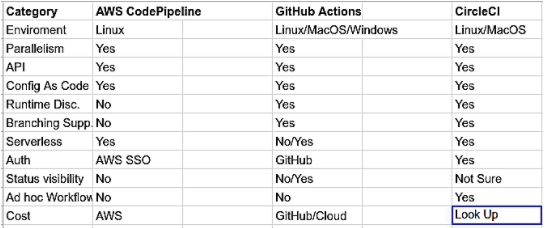
\includegraphics[width=7cm, height=7cm]{imagenes/tabla_comparativa.png}
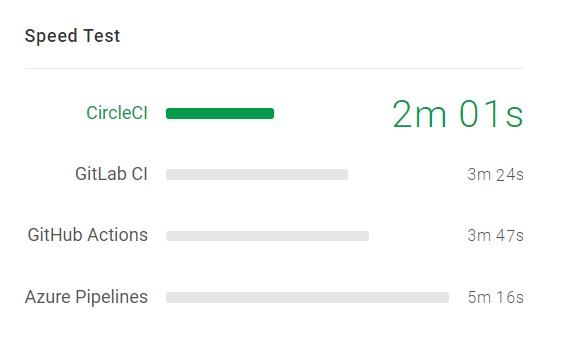
\includegraphics[width=7cm, height=7cm]{imagenes/comparativa.jpeg}
\subsubsection{Curva de aprendizaje}
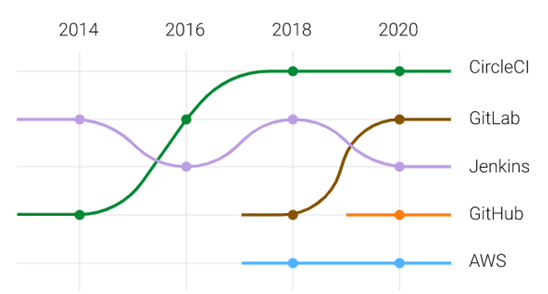
\includegraphics[width=7cm, height=7cm]{imagenes/curva.png}
Fuente: https://circleci.com/circleci-versus-github-actions/ 
\section{Conclusiones}
Las pruebas presentan información sobre la calidad del producto a las personas responsables de este. Las pruebas de calidad presentan los siguientes objetivos: encontrar defectos o bugs, aumentar la confianza en el nivel de calidad, facilitar información para la toma de decisiones, evitar la aparición de defectos.  
Teniendo esta afirmación en mente, la información que puede ser requerida es de lo más variada. Esto hace que el proceso de testing sea completamente dependiente del contexto en el que se desarrolla.  
El ambiente ideal de las pruebas es aquel que es independiente del desarrollo del software, de esta manera se logra objetividad en las pruebas.  
A pesar de lo que muchos promueven, no existen las "mejores prácticas" como tales. Toda práctica puede ser ideal para una situación, pero completamente inútil o incluso perjudicial en otra.  
Por esto, las actividades técnicas, documentación, enfoques y demás elementos que condicionarán las pruebas a realizar deben ser seleccionadas y utilizadas de la manera más eficiente según contexto del proyecto. 
\section{Recomendaciones}
El mercado está completamente cargado con varios productos de gestión de pruebas. Por lo tanto, encontrar la solución de gestión de pruebas adecuada para su organización se convierte en un proceso desafiante. 
\begin{itemize}
    \item 	Antes de comenzar a examinar las herramientas, es muy importante que comprenda las necesidades del proyecto. No continúe con una selección de herramientas sin saber exactamente qué está buscando y qué características espera de la herramienta. 
    \item 	Una vez que tenga claros los requisitos del proyecto, comience a evaluar las herramientas que se ajusten a su presupuesto y establezca las funciones según sus necesidades. 
    \item 	En lugar de optar por una sola herramienta, también puede tener la opción de optar por múltiples herramientas compatibles que juntas pueden servir como una solución de gestión de pruebas y satisfacer todas sus necesidades. 
    \item 	Lo siguiente que entra en consideración antes de profundizar en la función de la herramienta es su entorno de desarrollo. Las consultas relacionadas con la privacidad, seguridad, soporte de administración de TI, hosting, costo de mantenimiento, etc. con la nueva herramienta deben ser atendidas adecuadamente. 
    \item 	Además, debe considerar todos los problemas técnicos de los que debe ocuparse si va a utilizar una nueva herramienta. 
    \item 	Ahora, debe considerar las funciones de administración de pruebas que ofrece la herramienta. Compruebe si la herramienta ofrece todas las funciones básicas esenciales necesarias para la gestión de pruebas. 
  \item 	Continuando, si ya está utilizando una herramienta de gestión de defectos y desea continuar con ella, compruebe si la nueva herramienta se integra bien con su sistema de gestión de defectos. Esto es necesario para informar y realizar un seguimiento de los defectos correctamente. 
    \item 	Cualquiera que sea la herramienta o el conjunto de herramientas que elija, debe poder establecer una conexión entre los requisitos funcionales y los casos de prueba.  
\end{itemize}

%----------------------------------------------------------------------------------------
%	REFERENCE LIST
%----------------------------------------------------------------------------------------

\begin{thebibliography}{XXX0000}
	
\bibitem - 10 herramientas para la gestión de calidad de software. PMOinformatica.com (2012-2018). Recuperado de:  http://www.pmoinformatica.com/2015/04/herramientas-gestion-calidad-software.html
	\bibitem -Análisis y comparativa de herramientas de gestión de pruebas de uso gratuito. JavierGarzas.com (2021). Recuperado de: https://www.javiergarzas.com/2013/10/herramientas-de-gestion-de-pruebas.html 
    \bibitem -Herramienta de gestión de pruebas. Globe (2020). Recuperado de: https://www.globetesting.com/herramienta-de-gestion-de-pruebas/ 
    \bibitem -Esmite, I. Farías, M. Farías,  Pérez, (2007). Automatización y gestión de las pruebas funcionales usando herramientas open source. In XIII Congreso Argentino de Ciencias de la Computación. 
    \bibitem -Giang, n. t. p.,  khoa, t. t. m. (2020). automated continuous integration using circleci and firebase for android application development. journal of science and technology-iuh, 47(05).
    \bibitem -Kinsman, T., Wessel, M., Gerosa, M. A.,  Treude, C. (2021). How Do Software Developers Use GitHub Actions to Automate Their Workflows?. arXiv preprint arXiv:2103.12224. 
    \bibitem - Melgar Velásquez, R. (2020). Implementación de un modelo de gestión de pruebas de software según ISTQB para mejorar el proceso del área de certificación en tecnologías web de una entidad financiera.
    \bibitem -Pothecary, R. (2021). Developing on AWS. In Running Microsoft Workloads on AWS (pp. 111-138). Apress, Berkeley, CA.
	\end{thebibliography}

%----------------------------------------------------------------------------------------

\end{document}